\documentclass[a4paper,12pt]{article} % добавить leqno в [] для нумерации слева
\usepackage[a4paper,top=1.3cm,bottom=2cm,left=1.5cm,right=1.5cm,marginparwidth=0.75cm]{geometry}
%%% Работа с русским языком
\usepackage{cmap}					% поиск в PDF
\usepackage{mathtext} 				% русские буквы в фомулах
\usepackage[T2A]{fontenc}			% кодировка
\usepackage[utf8]{inputenc}			% кодировка исходного текста
\usepackage[english,russian]{babel}	% локализация и переносы
\usepackage{multirow}

\usepackage{graphicx}

\usepackage{wrapfig}
\usepackage{tabularx}

\usepackage{hyperref}
\usepackage[rgb]{xcolor}
\hypersetup{
colorlinks=true,urlcolor=blue
}

%%% Дополнительная работа с математикой
\usepackage{amsmath,amsfonts,amssymb,amsthm,mathtools} % AMS
\usepackage{icomma} % "Умная" запятая: $0,2$ --- число, $0, 2$ --- перечисление

%% Номера формул
\mathtoolsset{showonlyrefs=true} % Показывать номера только у тех формул, на которые есть \eqref{} в тексте.

%% Шрифты
\usepackage{euscript}	 % Шрифт Евклид
\usepackage{mathrsfs} % Красивый матшрифт

%% Свои команды
\DeclareMathOperator{\sgn}{\mathop{sgn}}

%% Перенос знаков в формулах (по Львовскому)
\newcommand*{\hm}[1]{#1\nobreak\discretionary{}
{\hbox{$\mathsurround=0pt #1$}}{}}

\date{\today}

\begin{document}

\begin{titlepage}
	\begin{center}
		{\large МОСКОВСКИЙ ФИЗИКО-ТЕХНИЧЕСКИЙ ИНСТИТУТ (НАЦИОНАЛЬНЫЙ ИССЛЕДОВАТЕЛЬСКИЙ УНИВЕРСИТЕТ)}
	\end{center}
	\begin{center}
		{\large Физтех-школа физики и исследований им. Ландау}
	\end{center}
	
	
	\vspace{4.5cm}
	{\huge
		\begin{center}
			{\bf Отчёт о выполнении лабораторной работы 1.4.1}\\
			Изучение физического маятника
		\end{center}
	}
	\vspace{2cm}
	\begin{flushright}
		{\LARGE Автор:\\ Сенокосов Арсений Олегович \\
			\vspace{0.2cm}
			Б02-012Б}
	\end{flushright}
	\vspace{8cm}
	\begin{center}
		Долгопрудный 2020
	\end{center}
\end{titlepage}

\section{Введение}

\textbf{Цель работы:} исследовать зависимость периода колебаний физического маятника от момента его инерции.\\
\textbf{В работе используются:} физический маятник (однородный стальной стержень), опорная призма, математический маятник, счётчик числа колебаний, линейка, секундомер.

\section{Теоретические сведения}

\begin{wrapfigure}{l}{6cm}
	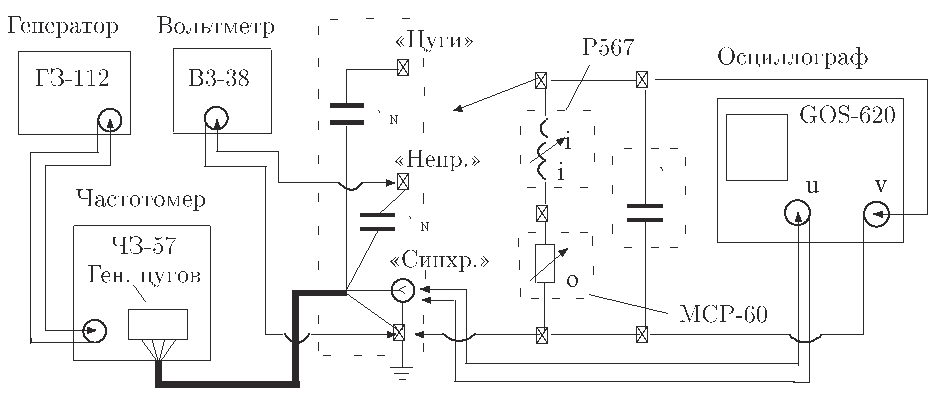
\includegraphics[width=1\linewidth]{ustanovka.png}
	\caption{Физический маятник}\label{risunok}
\end{wrapfigure}

Физическим маятником называют любое твердое тело, которое под действием силы тяжести может свободно качаться вокруг неподвижной горизонтальной оси. Движение маятника ­описывается уравнением

\begin{equation}
I\frac{d^2\varphi}{dt^2}=M,
\label{osnova}
\end{equation}

\noindent где $ I $ -- момент инерции маятника, $ \varphi $ -- угол отклонения маятника от положения равновесия, $ t $ - время, $ М $ - момент сил, действующих на маятник.

В данной работе в качестве физического маятника (рис.~ \ref{risunok}) используется однородный стальной стержень длиной $ l $. На стержне закрепляется опорная призма, острое ребро которой является осью качания маятника. Призму можно перемещать вдоль стержня, меняя таким образом расстояние $ OC $ от точки опоры маятника до его центра масс. Пусть это расстояние равно $ a $. Тогда по теореме Гюйгенса-Штейнера момент инерции маятника

\begin{equation}
I=\frac{ml^2}{12}+ma^2,
\end{equation}

\noindent где $ m $ -- масса маятника. Момент силы тяжести, действующий на маятник, 

\begin{equation}
M=-mga\sin\varphi.
\end{equation}

\noindent Если угол $ \varphi $ мал, то $ \sin\varphi\approx\varphi $, так что

\begin{equation}
M\approx-mga\varphi
\end{equation}

\noindent В исправной установке маятник совершает несколько сот колебаний без заметного затухания. Поэтому моментом силы трения в первом приближении можно пренебречь. Подставляя выражение для $ I $ и $ M $ в \eqref{osnova}, получим уравнение

\begin{equation}
\ddot{\varphi}+\omega^2\varphi=0,
\label{phi}
\end{equation}

\noindent где

\begin{equation}
\omega^2=\frac{ga}{a^2+\frac{l^2}{12}}.
\end{equation}

Тогда период колебаний равен

\begin{equation}\label{period}
T=\frac{2\pi}{\omega}=2\pi\sqrt{\frac{a^2+\frac{l^2}{12}}{ag}}
\end{equation}

Таким образом, период малых колебаний не зависит ни от начальной фазы, ни от амплитуды колебаний. Это утверждение (изохорность) справедливо для колебаний, подчиняющихся уравнению \eqref{phi}. Движение маятника описывается по этой формуле только для малых углов $ \varphi $.

\medskip

Период колебаний математического маятника определяется формулой
\begin{equation}
T'=2\pi\sqrt{\frac{l'}{g}},
\end{equation}
где $ l' $ -- длина математического маятника. Поэтому величину
\begin{equation}\label{prived}
l_\text{пр}=a+\frac{l^2}{12a}
\end{equation}
называют приведённой длиной математического маятника. Поэтому точку $ O' $ (см. рис. \ref{risunok}), отстоящую от точки опоры на расстояние $ l_\text{пр} $, называют центром качания физического маятника. Точка опоры и центр качания маятника обратимы, т.е. при качании маятника вокруг  точки $ O' $ период будет таким же, как и при качании вокруг точки $ O $.

\section{Оборудование и экспериментальные погрешности}

\textbf{Секундомер:} $ \Delta_c = 0,01 \text{ с}$\\
\textbf{Линейка:} $ \Delta_\text{лин} = 0,05 \text{ см}$

\section{Результаты измерений и обработка данных}
\subsection{Определение диапазона амплитуд, в пределах которых период колебаний маятника можно считать не зависящим от амплитуды}\label{formuli}

Определим диапазон амплитуд, в пределах которым колебания можно считать не зависящими от начальной фазы. Для этого отклоняем маятник на угол $ \varphi \approx 10^\circ  $ и измеряем период колебаний. Затем уменьшаем угол отклонения в 2 раза и повторяем измерения. Результаты приведены в таблице \ref{tab1}.

\begin{table}[h!]
	\begin{center}
		\begin{tabular}{|c|c|c|c|c|c|c|c|}
		\hline
		№ & $ \varphi $ & $ T_\text{общ} $, с & $ N_\text{изм} $ & $ T $, с   & $ T_\text{ср} $, с     & $ \sigma $, с     & $\varepsilon$, $ \% $       \\ \hline
		1 & 10 & 152,94    & 100        & 1,5294 &          &          &             \\ \cline{1-5}
		2 & 10 & 152,89    & 100        & 1,5289 & 1,5291 & 0,0001 & 0,0115 \\ \cline{1-5}
		3 & 10 & 152,91    & 100        & 1,5291 &          &          &             \\ \hline
		4 & 5  & 152,84    & 100        & 1,5284 &          &          &             \\ \cline{1-5}
		5 & 5  & 152,81    & 100        & 1,5281 & 1,5284 & 0,0002 & 0,0148 \\ \cline{1-5}
		6 & 5  & 152,88    & 100        & 1,5288 &          &          &             \\ \hline
	\end{tabular}
	\end{center}
	\caption{Результаты измерения периода колебаний в зависимости от начального угла}
\label{tab1}
\end{table}

Время одного колебания для отдельного эксперимента рассчитываем по формуле:

\begin{equation}
T=\frac{T_\text{общ}}{N_\text{изм}},
\end{equation}
где $ T_\text{общ} $ -- время $ N_\text{изм} $ колебаний.

Среднее значение периода колебаний для одной серии опытов рассчитываем по следующей формуле:

\begin{equation}
T_\text{ср}=\frac{1}{N_\text{изм}}\sum_{i=1}^{N_\text{изм}}T_i.
\end{equation}

Случайная погрешность определения $ T_\text{ср} $ вычисляется по формуле:

\begin{equation}
\sigma_\text{сл}=\sqrt{\frac{1}{N_\text{изм}\left( N_\text{изм} - 1 \right)}\sum_{i=1}^{N_\text{изм}}\left( T_\text{ср} - T_i \right)^2 }.
\end{equation}

Полная погрешность измерения периода колебаний в одной серии опытов определяется следующим соотношением:

\begin{equation}
\sigma = \sqrt{\Delta_\text{с}^2+\sigma_\text{сл}^2}.
\end{equation}

Также можем рассчитать относительную погрешность:

\begin{equation}
\varepsilon = \frac{\sigma}{T_\text{ср}}.
\end{equation}

Исходя из измерений и пользуясь представленными выше формулами, получаем, что\\ $  T_{10^\circ} =\left( 1,5291 \pm 0,0001\right)  $ с и $ T_{5^\circ} =\left(  1,5284 \pm 0,0002\right)  $ с. Следовательно, полученные значения периода колебаний маятника совпадают с хорошей точностью. Поэтому в дальнейшем будем считать колебания не зависящими от начальной фазы при отклонении на угол не более $ \varphi_0 \approx 5^\circ$.

\subsection{Вычисление ускорения свободного падения и длины стержня}

Для вычисления ускорения свободного падения и длины стержня будем исследовать зависимость периода колебаний $ T $ от расстояния $ a $ между точкой опоры и центром масс. Результаты проведённых измерений представлены в таблице \ref{tab2}.

\begin{table}[h!!]
	\begin{center}
		\begin{tabular}{|c|c|c|c|c|c|c|c|c|c|}
		\hline
		№ &
		$ a $, см &
		$ T_\text{общ} $, с &
		$ N_\text{изм} $ &
		$ T $, с &
		$ T_\text{ср} $, с &
		$ \Delta $, с &
		$ \sigma_\text{сл} $, с &
		$ \sigma_T$, с &
		$ \varepsilon $, $ \% $ \\ \hline
		1 &
		5 &
		132,47 &
		50 &
		2,6494 &
		\multirow{2}{*}{2,6503} &
		\multirow{2}{*}{0,0002} &
		\multirow{2}{*}{0,000129} &
		\multirow{2}{*}{0,0002} &
		\multirow{2}{*}{0,0089} \\ \cline{1-5}
		2 &
		5 &
		132,56 &
		50 &
		2,6512 &
		&
		&
		&
		&
		\\ \hline
		3 &
		10 &
		116,72 &
		60 &
		1,9453 &
		\multirow{2}{*}{1,9450} &
		\multirow{2}{*}{0,0001} &
		\multirow{2}{*}{$3,25 \cdot 10^{-5}$} &
		\multirow{2}{*}{0,0002} &
		\multirow{2}{*}{0,0087} \\ \cline{1-5}
		4 &
		10 &
		116,69 &
		60 &
		1,9448 &
		&
		&
		&
		&
		\\ \hline
		5 &
		15 &
		118,38 &
		70 &
		1,6911 &
		\multirow{2}{*}{1,6909} &
		\multirow{2}{*}{0,0001} &
		\multirow{2}{*}{$3,44 \cdot 10^{-5}$} &
		\multirow{2}{*}{0,0001} &
		\multirow{2}{*}{0,0086} \\ \cline{1-5}
		6 &
		15 &
		118,34 &
		70 &
		1,6905 &
		&
		&
		&
		&
		\\ \hline
		7 &
		20 &
		126,32 &
		80 &
		1,5791 &
		\multirow{2}{*}{1,5793} &
		\multirow{2}{*}{0,0001} &
		\multirow{2}{*}{$3,52 \cdot 10^{-5}$} &
		\multirow{2}{*}{0,0001} &
		\multirow{2}{*}{0,0082} \\ \cline{1-5}
		8 &
		20 &
		126,37 &
		80 &
		1,5796 &
		&
		&
		&
		&
		\\ \hline
		9 &
		25 &
		138,19 &
		90 &
		1,5354 &
		\multirow{2}{*}{1,5354} &
		\multirow{2}{*}{0,0001} &
		\multirow{2}{*}{$5,89 \cdot 10^{-6}$} &
		\multirow{2}{*}{0,0001} &
		\multirow{2}{*}{0,0072} \\ \cline{1-5}
		10 &
		25 &
		138,18 &
		90 &
		1,5353 &
		&
		&
		&
		&
		\\ \hline
		11 &
		28 &
		137,59 &
		90 &
		1,5287 &
		\multirow{2}{*}{1,5281} &
		\multirow{2}{*}{0,0001} &
		\multirow{2}{*}{$7,07 \cdot 10^{-5}$} &
		\multirow{2}{*}{0,0001} &
		\multirow{2}{*}{0,0086} \\ \cline{1-5}
		12 &
		28 &
		137,47 &
		90 &
		1,5274 &
		&
		&
		&
		&
		\\ \hline
		13 &
		30 &
		152,84 &
		100 &
		1,5284 &
		\multirow{2}{*}{1,5281} &
		\multirow{2}{*}{0,0001} &
		\multirow{2}{*}{$3,03 \cdot 10^{-5}$} &
		\multirow{2}{*}{0,0001} &
		\multirow{2}{*}{0,0068} \\ \cline{1-5}
		14 &
		30 &
		152,78 &
		100 &
		1,5278 &
		&
		&
		&
		&
		\\ \hline
		15 &
		33 &
		153,31 &
		100 &
		1,5331 &
		\multirow{2}{*}{1,5337} &
		\multirow{2}{*}{0,0001} &
		\multirow{2}{*}{$6,53 \cdot 10^{-5}$} &
		\multirow{2}{*}{0,0001} &
		\multirow{2}{*}{0,0077} \\ \cline{1-5}
		16 &
		33 &
		153,44 &
		100 &
		1,5344 &
		&
		&
		&
		&
		\\ \hline
		17 &
		35 &
		123,35 &
		80 &
		1,5418 &
		\multirow{2}{*}{1,5422} &
		\multirow{2}{*}{0,0001} &
		\multirow{2}{*}{$3,52 \cdot 10^{-5}$} &
		\multirow{2}{*}{0,0001} &
		\multirow{2}{*}{0,0084} \\ \cline{1-5}
		18 &
		35 &
		123,4 &
		80 &
		1,5425 &
		&
		&
		&
		&
		\\ \hline
		19 &
		37 &
		93,04 &
		60 &
		1,5506 &
		\multirow{2}{*}{1,5506} &
		\multirow{2}{*}{0,0001} &
		\multirow{2}{*}{$1,08 \cdot 10^{-5}$} &
		\multirow{2}{*}{0,0002} &
		\multirow{2}{*}{0,0108} \\ \cline{1-5}
		20 &
		37 &
		93,03 &
		60 &
		1,5505 &
		&
		&
		&
		&
		\\ \hline
	\end{tabular}
	\end{center}
\caption{Измерение периода колебаний маятника $ T $ в зависимости от расстояния $ a $}
\label{tab2}
\end{table}

По полученным данным вычисляем $ T $, $ T_\text{ср} $, $ \Delta $, $ \sigma_\text{сл}$, $ \sigma $ и $ \varepsilon $ по формулам представленным в разделе \ref{formuli}.

Используя формулу для периода физического маятника \eqref{period} получаем следующее соотношение:

\begin{equation}
T^2a=\frac{4\pi^2}{g}a^2+\frac{\pi^2l^2}{3g}.
\end{equation}
Отсюда можно сделать вывод о том, что $ T^2a $ линейно зависит от $ a^2 $, поэтому это зависимость можно представить в виде

\begin{equation}
T^2a=ka^2+b,
\end{equation}
где
\begin{equation}\label{koef}
k=\frac{4\pi^2}{g}  \text{ и }  b = \frac{\pi^2l^2}{3g}.
\end{equation}

Найдём эти коэффициента. Для удобства перенесём все необходимые данные в таблицу \ref{tab3}.

\begin{table}[h!]
	\begin{tabular}{|c|c|c|c|c|c|c|c|c|c|c|}
		\hline
		$ a $, см           & 5      & 10     & 15     & 20     & 25     & 28     & 30     & 33     & 35     & 37     \\ \hline
		$ a^2 $, $ \text{см}^2 $  & 25     & 100    & 225    & 400    & 625    & 784    & 900    & 1089   & 1225   & 1369   \\ \hline
		$ \sigma_{a^2}$,$ \text{см}^2  $         & 0,5    & 1      & 1,5    & 2      & 2,5    & 2,8    & 3      & 3,3    & 3,5    & 3,7    \\ \hline
		$ \varepsilon_{a^2}$ , $ \% $         & 2    & 1      & 0,67    & 0,5      & 0,4    & 0,36    & 0,33      & 0,31    & 0,28    & 0,27    \\ \hline
		$ T $, с           & 2,650  & 1,945  & 1,691  & 1,579  & 1,535  & 1,528  & 1,528  & 1,534  & 1,542  & 1,551  \\ \hline
		$ T^2 $, $ \text{с}^2 $   & 7,024  & 3,783  & 2,859  & 2,494  & 2,357  & 2,335  & 2,335  & 2,352  & 2,378  & 2,404  \\ \hline
		$ aT^2 $, $ \text{см} \cdot \text{с}^2 $ & 35,120 & 37,833 & 42,885 & 49,885 & 58,935 & 65,383 & 70,053 & 77,629 & 83,242 & 88,959 \\ \hline
		$ \sigma_{aT^2} $, $ \text{см} \cdot \text{с}^2  $       & 0,351  & 0,189  & 0,143  & 0,125  & 0,118  & 0,117  & 0,117  & 0,118  & 0,120  & 0,122  \\ \hline
		$ \varepsilon_{aT^2} $, $ \% $       & 1  & 0,5  & 0,33  & 0,25  & 0,21  & 0,18  & 0,16  & 0,15  & 0,14  & 0,3  \\ \hline
	\end{tabular}
\caption{Значения $ aT^2 $ и $ a^2 $ и их погрешности}
\label{tab3}
\end{table}

График зависимости $ aT^2 $ от $ a^2 $ представлен на рисунке \ref{graph}.

\begin{figure}[h!]
	\includegraphics[scale=0.38]{graph_file.jpeg}
	\caption{Зависимость $ aT^2 $ от $ a^2 $}
	\label{graph}
\end{figure}

Погрешность расчёта $ a^2 $ найдём по следующей формуле:

\begin{equation}
\sigma_{a^2}=2a^2\frac{\Delta a}{a}=2a\Delta a,
\end{equation}
где $ \Delta a = \Delta_\text{с} = 0,05$ см.

Погрешность вычисления $ aT^2 $ можно найти по формуле:

\begin{equation}
\sigma_{aT^2} = \sqrt{\left(  \frac{\Delta a}{a} \right)^2 + \left( 2\frac{\Delta T}{T} \right)^2 },
\end{equation}
где $ \Delta T = \sigma_T $ из таблицы \ref{tab2}.

Для вычисления коэффициентов $ k $ и $ b $ из \eqref{koef} воспользуемся методом наименьших квадратов:

\begin{equation}
k=\frac{\langle xy\rangle-\langle x\rangle \langle y\rangle}{\langle x^2\rangle - \langle x\rangle^2}\approx 0,04
02\text{ }\frac{\text{с}^2}{\text{см}},
\end{equation}

\begin{equation}
b=\langle y \rangle -k\langle x \rangle\approx 33,88\text{ }\text{см}\cdot\text{с}^2,
\end{equation}
где $ x=a^2 $, $ y=aT^2 $.

Случайные погрешности вычисления $ k $ и $ b $ можно найти по следующим формулам:

\begin{equation}
\sigma_k^\text{сл}=\sqrt{\frac{1}{N-2}\left(\frac{\langle y^2 \rangle - \langle y \rangle^2}{\langle x^2 \rangle - \langle x \rangle^2} - k^2 \right) } \approx 7,31 \cdot 10^{-5} \text{ }\frac{\text{с}^2}{\text{см}},
\end{equation}

\begin{equation}
\sigma_b^\text{сл}= \sigma_k^\text{сл} \sqrt{\langle x^2 \rangle - \langle x \rangle^2} \approx 0,0331 \text{ }\text{см}\cdot\text{с}^2.
\end{equation}

Систематическая погрешность вычисления коэффициентов определяется следующим соотношением:

\begin{equation}
\sigma^\text{сист}_k = k\sqrt{\left( \varepsilon_{aT^2} \right)^2 + \left( \varepsilon_{a^2} \right)^2 } \approx 0,0001 \text{ }\frac{\text{с}^2}{\text{см}},
\end{equation}

\begin{equation}
\sigma^\text{сист}_b = b\sqrt{\left( \varepsilon_{aT^2} \right)^2 + \left( \varepsilon_{a^2} \right)^2 } \approx  0,1026 \text{ }\text{см}\cdot\text{с}^2.
\end{equation}

Тогда полную погрешность вычисления коэффициентов подсчитываем по следующей формуле:

\begin{equation}
\sigma_k = \sqrt{\left( \sigma_k^\text{сл} \right)^2 + \left( \sigma_k^\text{сист} \right)^2 } \approx 0,0001 \text{ }\frac{\text{с}^2}{\text{см}},
\end{equation}

\begin{equation}
\sigma_b = \sqrt{\left( \sigma_b^\text{сл} \right)^2 + \left( \sigma_b^\text{сист} \right)^2 } \approx 0,1078 \text{ }\text{см}\cdot\text{с}^2.
\end{equation}

Таким образом, получаем:
\begin{itemize}
	\item $ k = \left( 0,0402\pm0,0001\right)  \text{ }\frac{\text{с}^2}{\text{см}} $, $ \varepsilon_k = 0,35 \% $
	\item $ b = \left( 33,88\pm0,11\right)  \text{ }\text{см}\cdot\text{с}^2 $, $ \varepsilon_b = 0,31 \% $
\end{itemize}

Учитывая формулу \eqref{koef}, вычисляем $ g $ и $ l $:

\begin{equation}
g = \frac{4\pi^2}{k} \approx 9,82 \text{ }\frac{\text{м}}{\text{с}^2},
\end{equation}

\begin{equation}
\sigma_g = g\cdot\varepsilon_k \approx 0,03 \text{ }\frac{\text{м}}{\text{с}^2},
\end{equation}

\begin{equation}
l=\sqrt{\frac{3bg}{\pi^2}}\approx 1,005 \text{ м},
\end{equation}

\begin{equation}
\sigma_l = l\sqrt{\left( \frac{1}{2}\varepsilon_b \right)^2 + \left( \frac{1}{2}\varepsilon_g \right)^2 }\approx 0,002 \text{ м}.
\end{equation}

В итоге имеем следующие результаты:

\begin{itemize}
	\item \underline{$ g = \left( 9,82\pm0,03\right) \frac{\text{м}}{\text{с}^2} $, $ \varepsilon_g=0,31\% $}
	\item \underline{$ l = \left( 1,005\pm0,002\right) \text{м} $, $ \varepsilon_l=0,2\% $}
\end{itemize}

\subsection{Проверка справедливости формулы приведённой длины физического маятника}

Для \textit{$ a = 25 $ см} подберём длину математического маятника, чтобы периоды колебаний совпадали. Возьмём \textit{$ l_\text{мат} = 58 $ см}. Запишем в таблицу \ref{tab_mat} результаты измерения периода колебаний математического маятника.


\begin{table}[h!]
	\begin{center}
		\begin{tabular}{|c|c|c|c|c|c|c|c|}
		\hline
		№ & $ l_\text{мат} $, см & $ T_\text{общ} $, с & $ N_\text{изм} $ & $ T_1 $, с   & $ T_\text{ср} $, с                     & $ \sigma $, с                     & $ \varepsilon, \% $                     \\ \hline
		1 & 58       & 122,44    & 80         & 1,5305 & \multirow{2}{*}{1,5298} & \multirow{2}{*}{0,0006} & \multirow{2}{*}{0,0417} \\ \cline{1-5}
		2 & 58       & 122,34    & 80         & 1,5293 &                         &                         &                         \\ \hline
	\end{tabular}
	\end{center}
\caption{Период колебаний математического маятника длиной $ l_\text{мат} = 58 $ см}
\label{tab_mat}
\end{table}

Получаем, что \underline{$ T_\text{ср}^\text{мат} = \left( 1,5305\pm0,0006 \right)  $ с} при $ l_\text{мат}=58 $ см.

Это значение с хорошей точностью совпадает с периодом колебаний физического маятника \underline{$ T_\text{ср}^\text{физ} = \left( 1,5354\pm0,0001 \right)  $ с} при $ a = 25 $ см.

Вычислим $ l_\text{пр} $ для $ a = 25 $ см по формуле \eqref{prived}:

\begin{equation}
l_\text{пр}=a+\frac{l^2}{12a}\approx 58,3 \text{ см}.
\end{equation}
Таким образом, $ l_\text{мат}\approx l_\text{пр} $ и формула приведённой длины физического маятника справедлива.

\subsection{Проверка обратимости точки подвеса и центра качания физического маятника}

Для $ a_1 = 25 $ см вычислим $ l_\text{пр} $:

\begin{equation}
l_\text{пр}=a_1+\frac{l^2}{12a_1}\approx 58,3 \text{ см}.
\end{equation}
Следовательно расстояние от центра масс до центра качания $ a_2 $ вычисляем следующим образом:
\begin{equation}
a_2=\left|a_1-l_\text{пр}\right|\approx 33 \text{ см}
\end{equation}

\begin{table}[h!]
	\begin{center}
		\begin{tabular}{|c|c|c|c|c|c|c|c|}
			\hline
			№ & $ a $, см & $ T_\text{общ} $, с & $ N_\text{изм} $ & $ T_1 $, с  & $ T_\text{ср} $, с               & $ \sigma_T $, с                & $ \varepsilon,\% $                \\ \hline
			1 & 25    & 138,19    & 90         & 1,5354 & \multirow{2}{*}{1,5354} & \multirow{2}{*}{0,0001} & \multirow{2}{*}{$ 0,007$} \\ \cline{1-5}
			2 & 25    & 138,18    & 90         & 1,5353 &                         &                         &                              \\ \hline \hline
			1 & 33    & 153,31    & 100        & 1,5331 & \multirow{2}{*}{1,5336} & \multirow{2}{*}{0,0001} & \multirow{2}{*}{$ 0,008$} \\ \cline{1-5}
			2 & 33    & 153,44    & 100        & 1,5344 &                         &                         &                              \\ \hline
		\end{tabular}
	\end{center}
\caption{Измерение периода колебаний физического маятника для $ a_1=25 $ см и $ a_2=33 $ см}\label{tab5}
\end{table}

Проведём измерение периода колебаний физического маятника для $ a_1=25 $ см и $ a_2=33 $ см. Результаты измерений представлены в таблице \ref{tab5}.\\

Получаем, что
\begin{itemize}
	\item \underline{$ T_{\text{ср}1} = \left( 1,5354\pm0,0001 \right) $ с}
	\item \underline{$ T_{\text{ср}2} = \left( 1,5336\pm0,0001 \right) $ с}
\end{itemize}
Следовательно, $ T_{\text{ср}1} \approx T_{\text{ср}2} $ и точка подвеса и центр качания физического маятника обратимы.

\section{Выводы и обсуждение результатов}

В ходе работы были получены следующие величины:
\begin{itemize}
	\item \underline{$ g = \left( 9,82\pm0,03\right) \frac{\text{м}}{\text{с}^2} $, $ \varepsilon_g=0,31\% $}
	\item \underline{$ l = \left( 1,005\pm0,002\right) \text{м} $, $ \varepsilon_l=0,2\% $}
\end{itemize}
Они были получены с хорошей точностью, что говорит о малых погрешностях при измерениях, а так же о хорошем методе нахождения этих величин.\\
Также, были экспериментально проверена теория о приведённой длине физического маятника и теория об обратимости точки подвеса и центра качания.
Точность полученных результатов можно повысить, если исключить ошибку при фиксации периода колебаний маятника, которая существует в силу неидеальной реакции экспериментатора. Возможно, стоит использовать цифровой прибор фиксации колебаний и отсчёта времени. Также свою погрешность вносит неточность определения расстояния от точки опоры до центра масс стержня.










\end{document}